\section{Fisher and Jeffreys: Two Roads Diverged in the Inference Forest}

\subsection{Probability Distributions and Estimation: From Frequencies to Inference}

If Venn grounded probability in long-run frequency, then \textbf{Ronald Fisher} took the next step: he built a mathematical language to extract structure from that frequency.

Where Venn saw probability as emerging from repeated trials, Fisher asked:  
\textit{How can we use that data to infer what we don’t yet know?}

In the early 20th century, this marked a shift — from observing patterns to estimating parameters, from counting outcomes to modeling distributions. Probability was no longer just a description of observed regularities. It became a method for learning:  
\textbf{What can data tell us about the world we cannot directly observe?}

\medskip

While Kolmogorov was formalizing the axioms of probability on a foundation of measure theory, Fisher and contemporaries like \textbf{Harold Jeffreys} were too busy solving real-world problems to wait for philosophical purity.

Their concern wasn’t whether a set was measurable. It was:

\begin{itemize}
    \item How do you estimate an unknown quantity from noisy data?
    \item How do you design an experiment to reduce uncertainty?
    \item How do you choose between competing models of the world?
\end{itemize}

Fisher didn’t abandon Venn’s frequentism — he supercharged it. He introduced new tools:

\begin{itemize}
    \item \textbf{Probability distributions} to model the variability of outcomes.
    \item \textbf{Likelihood functions} to estimate parameters.
    \item \textbf{Sufficient statistics} to compress data without losing information.
\end{itemize}

Suppose we measure the temperature of a sensor and assume it follows a normal distribution with unknown mean \( \mu \) and known standard deviation \( \sigma \).  
The core question becomes:  
\textbf{Given the data, what is the best estimate of \( \mu \)?}

This wasn’t Laplace’s symmetry. It wasn’t Boole’s logic. It wasn’t even Venn’s frequency.

This was something new: \textbf{Inference from randomness}.

\medskip

In the next section, we’ll explore how Fisher formalized this process — turning observed data into estimates, and variability into precision — laying the groundwork for the modern science of statistical learning.


\subsection{Probability Distributions and Estimation: From Frequencies to Parameters}

Venn grounded probability in the long-run behavior of observed frequencies. Fisher took that vision and turned it into a mathematical engine of inference.

Where Venn said probability was the result of repetition, Fisher asked:  
\textit{Can we use those repetitions to estimate what we cannot see?}

Rather than modeling whole universes of outcomes, Fisher focused on **parameters** — the hidden numerical summaries that shape distributions. He introduced a powerful idea: use probability distributions not to describe our ignorance, but to extract **structure from randomness**.

\medskip

While Kolmogorov was formalizing the axioms of probability in terms of σ-algebras and measures, Fisher was more interested in practice: 
\begin{itemize}
    \item How do we estimate an unknown mean?
    \item How do we compare two treatments?
    \item How do we quantify uncertainty using data alone?
\end{itemize}

At the heart of this approach was a new object: the **likelihood function**. Instead of assigning probabilities to outcomes, Fisher flipped the perspective — treating the observed data as fixed, and the parameters as variables. The result was a formal method for finding the parameter value that made the data most probable.

\medskip

Suppose we measure the temperature of a sensor and assume it follows a normal distribution with unknown mean \( \mu \) and known standard deviation \( \sigma \). The key question becomes:  
\textbf{How do we estimate \( \mu \) from the data?}

\begin{figure}[H]
\centering
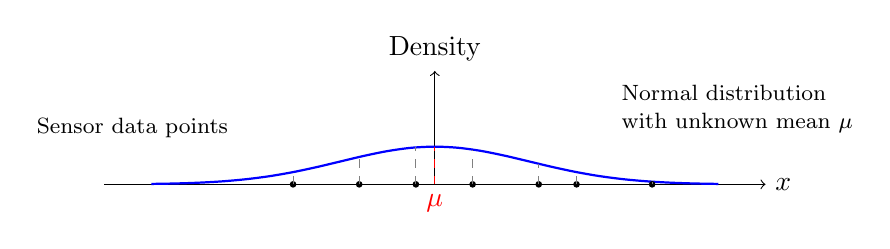
\begin{tikzpicture}[scale=1.2]
  % Axis
  \draw[->] (-3.5,0) -- (3.5,0) node[right] {$x$};
  \draw[->] (0,0) -- (0,1.2) node[above] {Density};

  % Normal distribution curve
  \draw[thick,domain=-3:3,smooth,variable=\x,blue] 
    plot ({\x},{exp(-(\x)^2/2)/sqrt(2*pi)});

  % True mean μ
  \draw[dashed,red] (0,0) -- (0,{exp(0)/sqrt(2*pi)});
  \node[below,red] at (0,0) {$\mu$};

  % Sample data points
  \foreach \x in {-1.5, -0.8, -0.2, 0.4, 1.1, 1.5, 2.3} {
    \fill[black] (\x,0) circle (1pt);
    \draw[gray, dashed] (\x,0) -- (\x,{exp(-(\x)^2/2)/sqrt(2*pi)});
  }

  % Annotation
  \node[align=left] at (3.2,0.8) {\footnotesize Normal distribution\\[-2pt] \footnotesize with unknown mean $\mu$};
  \node[align=center] at (-3.2,0.6) {\footnotesize Sensor data points};

\end{tikzpicture}
\caption{Estimating the mean \( \mu \) of a normal distribution from sensor data.}
\end{figure}

\begin{example}
Suppose we collect 10 temperature readings from a sensor:

\[
\{22.1, 21.8, 22.3, 21.9, 22.0, 21.7, 22.2, 22.1, 21.9, 22.0\}
\]

Assume the readings follow a normal distribution with known standard deviation \( \sigma = 0.2 \), but unknown mean \( \mu \). Our goal is to estimate \( \mu \).

\textbf{Fisher's Approach (Maximum Likelihood Estimation)}:  
We choose the value of \( \mu \) that maximizes the likelihood of observing the data. This leads to:

\[
\hat{\mu}_{\text{MLE}} = \frac{1}{n} \sum_{i=1}^{n} x_i = 22.0
\]
\end{example}

\subsubsection{A Laplacian Contrast: Belief as Distribution}

Fisher treated the parameter \( \mu \) as fixed but unknown — a quantity to be estimated from the data alone. But a century earlier, \textbf{Laplace} proposed a radically different view:  
\textbf{What if parameters were themselves uncertain quantities?}

In Laplace’s Bayesian framework, we model our ignorance about \( \mu \) with a probability distribution. We begin with a prior belief (say, that all values of \( \mu \) are equally likely), and then update that belief after seeing data.

If we assume a uniform prior for \( \mu \), the posterior distribution is:

\[
\mu \mid \text{data} \sim \mathcal{N}\left(\bar{x}, \frac{\sigma^2}{n}\right) = \mathcal{N}(22.0,\ 0.004)
\]

Where Fisher gave us the best estimate, Laplace gave us a distribution — not just a number, but a structured expression of our uncertainty.

\begin{quote}
\textit{Fisher estimated the world. Laplace updated belief about it.}
\end{quote}

\medskip

In the next sections, we’ll dive deeper into how Fisher’s approach — built on likelihood, sufficiency, and efficiency — shaped the practice of modern statistics, and how Laplace’s probabilistic logic lived on through Bayesian inference.



\subsection{The Estimator: Turning Data Into a Guess}

In Fisher’s world, data isn’t just observed — it’s leveraged. If probability tells us what outcomes are likely, an estimator tells us what parameters are plausible. It’s the mathematical bridge between raw samples and hidden structure.

Where Laplace gave us beliefs over parameters, Fisher gave us procedures for estimating them — directly, repeatably, and rigorously.

\medskip

Imagine you're trying to guess the average height of all the trees in a massive forest. You can’t measure every tree — there are millions. So instead, you take a walk, measure a handful, and try to make an educated guess.

That guess is called an \textbf{estimator}.

An estimator is a rule — a formula — that takes the data you have and produces a guess about what you can’t see. You don’t know the true average height \( \mu \), but based on your sample, you compute:

\[
\hat{\mu} = \frac{1}{n} \sum_{i=1}^n x_i
\]

Here, \( x_1, x_2, \dots, x_n \) are the observed tree heights, and \( \hat{\mu} \) is your estimate of the forest-wide average.

\begin{figure}[H]
\centering
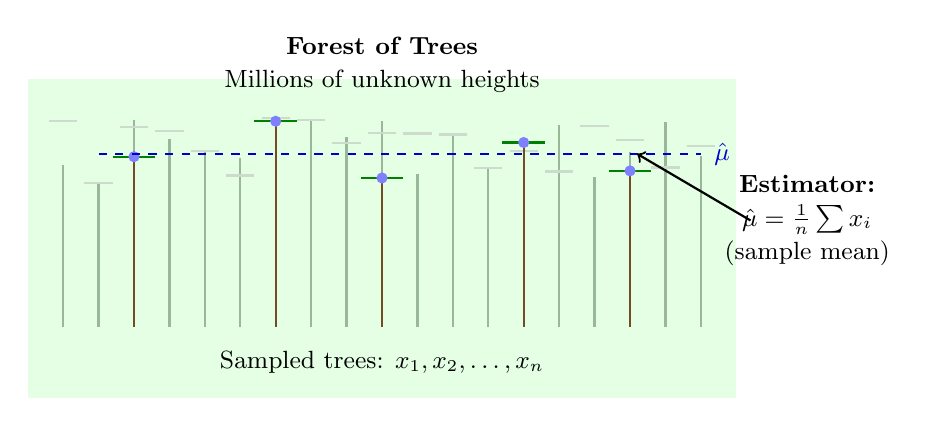
\begin{tikzpicture}[scale=0.9, every node/.style={font=\small}]

  % Forest background
  \fill[green!10] (-5,-1) rectangle (5,3.5);

  % Draw many trees in background (faint)
  \foreach \x in {-4.5,-4,...,4.5} {
    \draw[green!30!black!40, thick] (\x,0) --++ (0,2.5+rand*0.5);
    \draw[green!30!black!20, thick] (\x-0.2,2.5+rand*0.5) --++ (0.4,0);
  }

  % Highlighted sample trees
  \foreach \x/\h in {-3.5/2.4, -1.5/2.9, 0/2.1, 2/2.6, 3.5/2.2} {
    \draw[brown!60!black, thick] (\x,0) --++ (0,\h);
    \draw[green!50!black, thick] (\x-0.3,\h) --++ (0.6,0);
    \filldraw[blue!50] (\x,\h) circle (2pt);
  }

  % Sample mean line
  \draw[dashed,blue!80!black, thick] (-4,2.44) -- (4.5,2.44);
  \node[blue!80!black] at (4.8,2.44) {$\hat{\mu}$};

  % Label for sample
  \node at (0,-0.5) {Sampled trees: \( x_1, x_2, \dots, x_n \)};

  % Forest label
  \node[align=center] at (0,3.7) {\textbf{Forest of Trees}\\[1pt] Millions of unknown heights};

  % Estimator annotation
  \node[align=center] at (6,1.5) {\textbf{Estimator:}\\[1pt]
  \( \hat{\mu} = \frac{1}{n} \sum x_i \)\\[1pt] 
  (sample mean)};

  \draw[->, thick] (5.2,1.5) -- (3.6,2.44);

\end{tikzpicture}
\caption{Using a sample of tree heights to estimate the true forest-wide average.}
\end{figure}

\medskip

But here’s the twist: \textbf{your estimate is random}. If someone else took a different path through the forest and sampled different trees, they’d get a different \( \hat{\mu} \). The estimator isn’t just a number — it’s a \textit{random variable}, whose variability reflects the randomness of sampling itself.

\begin{quote}
An estimator is like a recipe. The data are the ingredients. The outcome depends on what you’re handed.
\end{quote}

Fisher didn’t just define estimators — he evaluated them. He asked:

\begin{itemize}
    \item Does the estimator tend to get the right answer? (\textbf{Unbiasedness})
    \item How much does it vary from sample to sample? (\textbf{Variance})
    \item Is it the best we can possibly do, given the data and assumptions? (\textbf{Efficiency})
\end{itemize}

\begin{example}
Suppose we sample five students and record their sleep hours:

\[
x = \{6.5, 7, 8, 5.5, 7.5\}, \quad \hat{\mu} = 6.9
\]

A second sample might give:

\[
x' = \{6, 6.5, 7.5, 6, 7\}, \quad \hat{\mu}' = 6.6
\]

Same estimator, different data, different guess. Over many samples, the estimator would bounce around — but if it’s well-designed, the average of all those estimates would converge to the true value \( \mu \). That’s what makes it \textbf{unbiased} — and the amount of bounce is its \textbf{variance}.
\end{example}

\medskip

In the next section, we’ll explore how Fisher went beyond the estimator itself — asking how much information a sample contains about the unknown. Not all data is equally informative. And Fisher developed a way to measure that, too.




\subsection{Fisher’s World: Likelihoods and Information}

Fisher didn’t care about probabilities as degrees of belief. For him, probability was a model of how nature produces data. Once the data arrives, the job of statistics is to invert the process.

He introduced the \textbf{likelihood function}:

\[
\mathcal{L}(\theta) = P(\text{data} \mid \theta)
\]

This measures how likely a parameter \( \theta \) is to have generated the data. In Fisher’s world, the data is fixed and the parameter is unknown but \textit{not random}.

He also introduced the concept of \textbf{Fisher information}—a way to quantify how much information the data carries about the parameter:

\[
\mathcal{I}(\theta) = \mathbb{E}\left[ \left( \frac{\partial}{\partial \theta} \log P(X \mid \theta) \right)^2 \right]
\]

High Fisher information means sharper likelihoods—data that’s more decisive. This would go on to power everything from efficient estimators to the Cramér-Rao bound.

\begin{figure}[H]
\centering
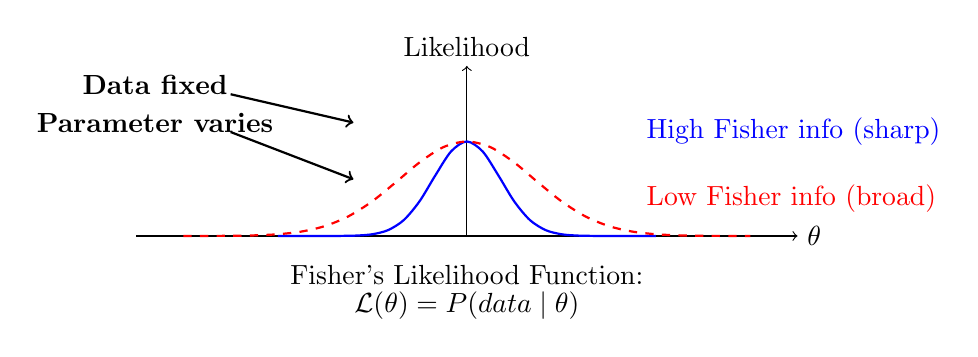
\begin{tikzpicture}[scale=1.2]
  % Axes
  \draw[->] (-3.5,0) -- (3.5,0) node[right] {$\theta$};
  \draw[->] (0,0) -- (0,1.8) node[above] {Likelihood};

  % High Fisher information (sharp peak)
  \draw[thick,blue,domain=-2:2,smooth,variable=\x] 
    plot ({\x},{exp(-4*(\x)^2)});

  % Low Fisher information (broad peak)
  \draw[thick,red,dashed,domain=-3:3,smooth,variable=\x] 
    plot ({\x},{exp(-(\x)^2)});

  % Labels
  \node[blue,right] at (1.8,1.1) {High Fisher info (sharp)};
  \node[red,right] at (1.8,0.4) {Low Fisher info (broad)};

  % Data fixed arrow
  \node at (-3.3,1.6) {\textbf{Data fixed}};
  \draw[->, thick] (-2.5,1.5) -- (-1.2,1.2);

  % Parameter θ varies arrow
  \node at (-3.3,1.2) {\textbf{Parameter varies}};
  \draw[->, thick] (-2.5,1.1) -- (-1.2,0.6);

  % Annotation
  \node[align=center] at (0,-0.6) {
    Fisher’s Likelihood Function: \\[-2pt]
    \( \mathcal{L}(\theta) = P(\text{data} \mid \theta) \)
  };

\end{tikzpicture}
\caption{In Fisher’s view, data is fixed and the likelihood is a function of the parameter \( \theta \). The sharper the peak, the more information the data carries about \( \theta \).}
\end{figure}


\subsubsection{A Worked Example: Likelihood and Fisher Information in Action}

Imagine you're studying radioactive particles, and you're measuring how long they take to decay. These decay times are unpredictable, but they follow a well-known pattern: the exponential distribution.

\[
f(x \mid \lambda) = \lambda e^{-\lambda x}, \quad x \geq 0
\]

Here, \( \lambda \) is the decay rate—how quickly things fall apart. And you're trying to estimate it from data. But you’ve only seen one decay event, and it happened at exactly \( x = 2 \) seconds.

\begin{figure}[H]
\centering
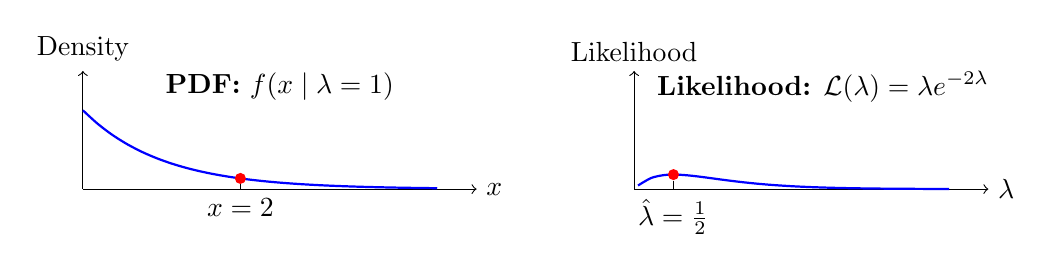
\begin{tikzpicture}

% Left plot: Exponential PDF with fixed lambda
\begin{scope}[scale=1]
  % Axes
  \draw[->] (0,0) -- (5,0) node[right] {$x$};
  \draw[->] (0,0) -- (0,1.5) node[above] {Density};

  % Exponential curve for lambda = 1
  \draw[thick,blue,domain=0:4.5,smooth,variable=\x] 
    plot ({\x},{exp(-\x)});

  % Mark x = 2
  \draw[dashed] (2,0) -- (2,{exp(-2)});
  \fill[red] (2,{exp(-2)}) circle (2pt);
  \node[below] at (2,0) {$x = 2$};

  % Label
  \node at (2.5,1.3) {\textbf{PDF:} \( f(x \mid \lambda = 1) \)};
\end{scope}

% Right plot: Likelihood as function of lambda
\begin{scope}[xshift=7cm,scale=1]
  % Axes
  \draw[->] (0,0) -- (4.5,0) node[right] {$\lambda$};
  \draw[->] (0,0) -- (0,1.5) node[above] {Likelihood};

  % Likelihood curve: L(lambda) = lambda * exp(-lambda * 2)
  \draw[thick,blue,domain=0.05:4,smooth,variable=\l] 
    plot ({\l},{\l*exp(-2*\l)});

  % Peak of the likelihood (at 1/2)
  \draw[dashed] ({1/2},0) -- ({1/2},{(1/2)*exp(-1)});
  \fill[red] ({1/2},{(1/2)*exp(-1)}) circle (2pt);
  \node[below] at (0.5,0) {$\hat{\lambda} = \frac{1}{2}$};

  % Label
  \node at (2.4,1.3) {\textbf{Likelihood:} \( \mathcal{L}(\lambda) = \lambda e^{-2\lambda} \)};
\end{scope}

\end{tikzpicture}
\caption{Left: PDF of exponential decay with \( \lambda = 1 \). Right: Likelihood of \( \lambda \) given observed decay at \( x = 2 \). The peak occurs at \( \hat{\lambda} = 1/2 \).}
\end{figure}


\vspace{0.5em}
\noindent
\textbf{Step 1: Likelihood—What Would Make This Observation Most Expected?}

The likelihood function tells you: if you assume a particular value of \( \lambda \), how plausible is it that you’d see a decay at 2 seconds?

\[
\mathcal{L}(\lambda) = \lambda e^{-2\lambda}
\]

This is like playing a game of “Guess the Parameter” where each guess gets a score based on how well it explains what you saw. The best guess—the one that makes your observation most likely—is the peak of this curve.

It turns out this peak is at:

\[
\hat{\lambda}_{\text{MLE}} = \frac{1}{2}
\]

So based on that one event at 2 seconds, your best guess is that the true decay rate is 0.5. Not certain—just most likely.


\begin{figure}[H]
\centering
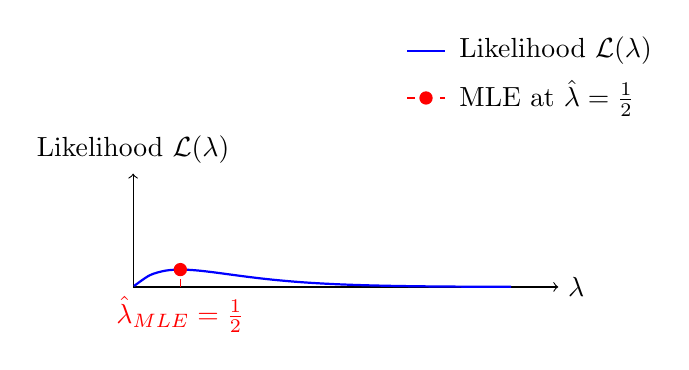
\begin{tikzpicture}[scale=1.2]

  % Axes
  \draw[->] (0,0) -- (4.5,0) node[right] {$\lambda$};
  \draw[->] (0,0) -- (0,1.2) node[above] {Likelihood \( \mathcal{L}(\lambda) \)};

  % Likelihood curve: L(lambda) = lambda * exp(-2*lambda)
  \draw[thick,blue,domain=0.01:4,smooth,variable=\l] 
    plot ({\l},{\l*exp(-2*\l)});

  % Peak at lambda = 0.5
  \draw[dashed,red] (0.5,0) -- (0.5,{0.5*exp(-1)});
  \fill[red] (0.5,{0.5*exp(-1)}) circle (2pt);
  \node[below,red] at (0.5,0) {\( \hat{\lambda}_{\text{MLE}} = \frac{1}{2} \)};

  % Legend box
  %\draw[fill=white, draw=black] (2.8,0.1) rectangle (4.2,0.6);

  % Legend entries
  \draw[thick,blue] (2.9,2.5) -- (3.3,2.5);
  \node[right] at (3.35,2.5) {Likelihood \( \mathcal{L}(\lambda) \)};

  \draw[red,dashed] (2.9,2) -- (3.3,2);
  \fill[red] (3.1,2) circle (2pt);
  \node[right] at (3.35,2) {MLE at \( \hat{\lambda} = \frac{1}{2} \)};

\end{tikzpicture}
\caption{The likelihood function \( \mathcal{L}(\lambda) = \lambda e^{-2\lambda} \). The peak at \( \lambda = \frac{1}{2} \) is the MLE: the parameter value that makes observing a 2-second decay most plausible.}
\end{figure}




\vspace{0.5em}
\noindent
\textbf{Step 2: Fisher Information—How Sharp Is Your Guess?}

Fisher Information measures how much information your observation gives you about the parameter. In a way, it’s a sensitivity check: if small changes in \( \lambda \) make big changes in likelihood, then your data is highly informative. If the likelihood curve is flat and squishy, your data doesn’t help much.

For the exponential distribution, the Fisher information for one observation is:

\[
\mathcal{I}(\lambda) = \frac{1}{\lambda^2}
\]

Here’s what that means:

\begin{itemize}
    \item If \( \lambda = 0.5 \), then \( \mathcal{I} = 4 \): you get a sharp, confident estimate.
    \item If \( \lambda = 2 \), then \( \mathcal{I} = 0.25 \): the estimate is fuzzier.
\end{itemize}

\vspace{0.5em}
\noindent
\textbf{Conclusion:} When decay is slow, each observation is packed with information—you can see more of the “tail” of the distribution. But when decay is fast, it’s harder to learn anything from one quick blip. The Fisher information puts numbers on this intuition.






\begin{figure}[H]
\centering
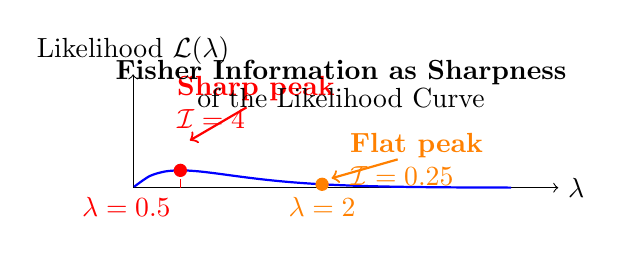
\begin{tikzpicture}[scale=1.2]

  % Axes
  \draw[->] (0,0) -- (4.5,0) node[right] {$\lambda$};
  \draw[->] (0,0) -- (0,1.2) node[above] {Likelihood \( \mathcal{L}(\lambda) \)};

  % Likelihood curve for x=2: L(lambda) = lambda * exp(-2*lambda)
  \draw[thick,blue,domain=0.01:4,smooth,variable=\l] 
    plot ({\l},{\l*exp(-2*\l)});

  % Highlight lambda = 0.5 (sharp)
  \draw[dashed,red] (0.5,0) -- (0.5,{0.5*exp(-1)});
  \fill[red] (0.5,{0.5*exp(-1)}) circle (2pt);
  \node[below left,red] at (0.5,0) {\( \lambda = 0.5 \)};
  \node[red,align=left] at (1.3,0.9) {\textbf{Sharp peak}\\\(\mathcal{I} = 4\)};
  \draw[->,red,thick] (1.2,0.85) -- (0.6,0.5);

  % Highlight lambda = 2 (flat)
  \draw[dashed,orange] (2,0) -- (2,{2*exp(-4)});
  \fill[orange] (2,{2*exp(-4)}) circle (2pt);
  \node[below,orange] at (2,0) {\( \lambda = 2 \)};
  \node[orange,align=left] at (3,0.3) {\textbf{Flat peak}\\\(\mathcal{I} = 0.25\)};
  \draw[->,orange,thick] (2.8,0.3) -- (2.1,0.1);

  % Title label
  \node[align=center] at (2.2,1.1) {
    \textbf{Fisher Information as Sharpness}\\[-2pt]
    of the Likelihood Curve
  };

\end{tikzpicture}
\caption{Sharper likelihoods (e.g., at \( \lambda = 0.5 \)) imply more Fisher information. Flatter likelihoods (e.g., at \( \lambda = 2 \)) imply less. Fisher information quantifies how much your data narrows down the parameter.}
\end{figure}



\begin{tcolorbox}[title={\textbf{Historical Sidebar: Fisher, Smoking, and the Limits of Inference}}, colback=gray!5, colframe=black, fonttitle=\bfseries]

  \textbf{Ronald Fisher}, father of modern statistics, was famously skeptical that smoking caused cancer. In the 1950s, as epidemiological studies began to show strong correlations between smoking and lung cancer, Fisher dismissed the results -- not because he loved tobacco (though he did smoke a pipe), but because he didn’t think the \emph{math} justified the claim.

  \medskip
  
  Fisher argued that the statistical methods used --- particularly significance tests and \( p \)-values --- were being stretched beyond their limits. Correlation, he insisted, was not causation. He claimed that observed association might be due to some hidden third factor (what we now call a confounder). In fact, he once proposed that a genetic predisposition could lead both to smoking and to cancer.
  
  \medskip
  
  In hindsight, this seems absurd. The causal link between smoking and cancer is now one of the best established in all of medicine. However, from Fisher’s point of view, the statistical evidence alone wasn’t strong enough to justify a claim of causality. And, technically, he was right.
  
  \medskip
  
  The Moral? Even correct methods and analysis can lead you astray. Fisher demanded rigor; and, in doing so, he missed the obvious.
  
  \begin{quote}
    \textit{You can follow the rules perfectly and still end up perfectly wrong.}
  \end{quote}
    
  
\end{tcolorbox}

 
\subsection{Linear Regression: Estimation in the Spirit of Fisher}

For Fisher, statistics was about extracting reliable, efficient estimates from noisy data. \textbf{Linear regression} embodied this mission — using mathematical precision to reveal underlying structure.

\medskip

The model:

\[
y = X\beta + \varepsilon
\]

Where:
\begin{itemize}
    \item \( y \in \mathbb{R}^n \) is the vector of observations,
    \item \( X \in \mathbb{R}^{n \times p} \) is the matrix of predictors,
    \item \( \beta \in \mathbb{R}^p \) is the vector of unknown parameters,
    \item \( \varepsilon \sim \mathcal{N}(0, \sigma^2 I) \) represents random error.
\end{itemize}

The objective is clear:  
\textbf{Find the estimator \( \hat{\beta} \) that minimizes the sum of squared residuals.}

\[
\hat{\beta} = \arg\min_{\beta} \| y - X\beta \|^2
\]

This leads to the famous \textbf{normal equations}:

\[
X^\top X \hat{\beta} = X^\top y
\]

Provided \( X^\top X \) is invertible, the solution is:

\[
\hat{\beta} = (X^\top X)^{-1} X^\top y
\]

Fisher didn’t just derive estimators — he evaluated them. For him, an estimator wasn’t "good" simply because it produced a number. It had to meet strict mathematical criteria grounded in logic and efficiency. 

He assessed estimators like \( \hat{\beta} \) using three key properties:

\medskip

\paragraph{\textbf{Unbiasedness: Trusting the Long Run}}

An estimator \( \hat{\beta} \) is said to be \textbf{unbiased} if, on average, it hits the true parameter value:

\[
\mathbb{E}[\hat{\beta}] = \beta
\]

For linear regression, assuming the classical conditions (linearity, independence, homoscedasticity, no multicollinearity), we have:

\[
\hat{\beta} = (X^\top X)^{-1} X^\top y
\]

Substitute \( y = X\beta + \varepsilon \):

\[
\hat{\beta} = (X^\top X)^{-1} X^\top (X\beta + \varepsilon) = \beta + (X^\top X)^{-1} X^\top \varepsilon
\]

Taking expectations:

\[
\mathbb{E}[\hat{\beta}] = \beta + (X^\top X)^{-1} X^\top \mathbb{E}[\varepsilon]
\]

Since \( \mathbb{E}[\varepsilon] = 0 \), it follows that:

\[
\mathbb{E}[\hat{\beta}] = \beta
\]

\textbf{Interpretation:} If you repeated the experiment infinitely many times, the average of all your estimates would converge to the true parameter. For Fisher, this wasn’t just a technicality — it was a safeguard against systematic error.

\medskip

\paragraph{\textbf{Variance: Measuring the "Wobble"}}

While unbiasedness ensures you're aiming at the right target, variance tells you how tightly your shots cluster around it.

For \( \hat{\beta} \), the variance-covariance matrix is:

\[
\mathrm{Var}(\hat{\beta}) = \mathbb{E} \left[ (\hat{\beta} - \beta)(\hat{\beta} - \beta)^\top \right] = \sigma^2 (X^\top X)^{-1}
\]

Where \( \sigma^2 \) is the variance of the error term \( \varepsilon \).

\textbf{Key Insight:}  
If \( X^\top X \) is close to singular (i.e., predictors are correlated), the inverse \( (X^\top X)^{-1} \) becomes large — inflating the variance of \( \hat{\beta} \). This means:

- Your estimator is still \textit{correct on average},  
- But any single estimate could be wildly off due to high variability.

Fisher was deeply concerned with this tradeoff — knowing that an estimator with enormous variance, while technically unbiased, was practically useless.

\medskip

\paragraph{\textbf{Efficiency: The Best You Can Do (Within Reason)}}

Among all possible


\medskip

But even within this elegant framework, statisticians faced practical mathematical challenges — ones that modern hyperparameters now automate.

\medskip

\begin{tcolorbox}[title=\textbf{Mathematical Considerations: Fisher-Era Decisions}, colback=gray!5, colframe=black, fonttitle=\bfseries]

\vspace{-0.5em}

\paragraph{1. Controlling Complexity: Implicit Regularization}
If \( X^\top X \) is nearly singular (e.g., when predictors are highly correlated), the variance of \( \hat{\beta} \) explodes:

\[
\mathrm{Var}(\hat{\beta}) = \sigma^2 (X^\top X)^{-1}
\]

To stabilize estimates, statisticians could \emph{implicitly} constrain the solution — a precursor to what we now formalize as \textbf{Ridge Regression}:

\[
\hat{\beta}_{\text{ridge}} = (X^\top X + \lambda I)^{-1} X^\top y
\]

Here, \( \lambda > 0 \) shrinks coefficients, reducing variance at the cost of slight bias — a tradeoff Fisher would recognize as favoring **efficiency** over purity.

\medskip

\paragraph{2. Adjusting for Baselines: The Intercept Term}
If the data isn’t centered, omitting the intercept biases the estimate. Mathematically:

\[
y = X\beta + b + \varepsilon
\]

Including the intercept amounts to augmenting \( X \) with a column of ones:

\[
X' = 
\begin{bmatrix}
1 & x_{11} & \dots & x_{1p} \\
1 & x_{21} & \dots & x_{2p} \\
\vdots & \vdots & & \vdots \\
1 & x_{n1} & \dots & x_{np}
\end{bmatrix}
\]

Failing to include \( b \) when needed leads to systematic errors in \( \hat{\beta} \). Fisher’s emphasis on proper experimental design was, in part, about ensuring that such structural aspects were correctly specified.

\medskip

\paragraph{3. Solving the Normal Equations: A Matter of Feasibility}
While the formula for \( \hat{\beta} \) is compact, computing \( (X^\top X)^{-1} \) by hand was infeasible for large \( p \). Statisticians used methods like:

\begin{itemize}
    \item Exploiting symmetry of \( X^\top X \),
    \item Applying matrix factorizations (e.g., Cholesky, though formalized later),
    \item Reducing dimensionality through careful variable selection — another nod to complexity control.
\end{itemize}

These weren’t called "solvers," but they reflected the same challenge: \textbf{How do you compute stable estimates efficiently, given limited resources?}

\end{tcolorbox}

\medskip

Thus, even in Fisher’s era, the core concerns behind modern hyperparameters were alive and well — framed not as knobs for machine learning models, but as mathematical and philosophical judgments about inference, stability, and rigor.




\subsection{The Limits of Likelihood: When Inference Isn’t Enough}

Fisher gave us powerful tools to estimate parameters, quantify uncertainty, and design efficient experiments. But there was one question his framework was never built to answer:

\begin{center}
\textbf{Does X \emph{cause} Y?}
\end{center}

Likelihoods, estimators, and \( p \)-values can tell you whether an association exists, how strong it appears, and how likely it is to arise by chance. But they remain silent on the deeper issue of causality.

\medskip

Fisher’s skepticism about smoking and cancer wasn’t a misunderstanding of biology — it was a demonstration of the boundaries of his own mathematical creations. His methods could detect patterns, but they couldn’t distinguish:

\begin{itemize}
    \item Whether smoking \emph{causes} cancer,
    \item Whether cancer predisposition \emph{causes} smoking,
    \item Or whether both are driven by some hidden confounder.
\end{itemize}

To Fisher, claiming causality from correlation was statistical heresy — and by the rules of inference he helped invent, he wasn’t wrong.

\medskip

This exposes a crucial lesson:  
\textbf{Statistical inference is about estimating what is, not explaining why it is.}

Fisher’s framework excels when:
\begin{itemize}
    \item The model is known.
    \item The parameters are fixed but unknown.
    \item The goal is precision within a well-defined system.
\end{itemize}

But when the question shifts from \emph{estimation} to \emph{explanation}, from \emph{patterns} to \emph{processes}, likelihood-based inference starts to crack.

\medskip

\begin{tcolorbox}[colback=gray!5, colframe=black, title=\textbf{Correlation, Causation, and the Missing Toolkit}]
Fisher taught us how to measure uncertainty — but he didn’t give us tools to untangle cause and effect.

\textbf{Statistical inference asks:}  
\quad “Given this data, what parameters likely produced it?”

\textbf{Causal inference asks:}  
\quad “What happens if we intervene and change something?”

They are fundamentally different questions — and answering the second requires assumptions, frameworks, and methods that go beyond Fisher’s likelihoods.
\end{tcolorbox}

\medskip

It wasn’t until decades later that researchers like \textbf{Judea Pearl} began formalizing causal inference — introducing concepts like \textbf{do-calculus}, causal graphs, and counterfactual reasoning to address what Fisher’s generation avoided.

\medskip

\begin{quote}
\textit{Fisher mapped the terrain of uncertainty. But causality lives beyond that map.}
\end{quote}

In the next section, we’ll briefly explore how modern statistics and machine learning attempt to bridge this gap — and why knowing the limits of inference is just as important as knowing its power.

